% CS329H final manuscript (due Thu 3 Dec 2026). NeurIPS 2025 style, at most 8 pages excluding references.
% Every number below comes from code/results/ and every figure and table from code/scripts/make_figures.py.
\documentclass{article}

\usepackage[preprint]{../neurips_2025}
\makeatletter
\renewcommand{\@noticestring}{CS329H: Machine Learning from Human Preferences, Stanford University, Autumn 2026. Final project.}
\makeatother

\usepackage[utf8]{inputenc}
\usepackage[T1]{fontenc}
\usepackage{hyperref}
\hypersetup{colorlinks=true,linkcolor=black,citecolor=black,urlcolor=blue!60!black}
\usepackage{url}
\usepackage{booktabs}
\usepackage{tabularx}
\usepackage{amsfonts,amsmath,amssymb}
\usepackage{microtype}
\usepackage{xcolor}
\usepackage{graphicx}
\graphicspath{{../code/figures/}}

\title{Ask About Money, Keep the Questionnaire:\\What an AI Adviser Should Ask About Risk}

\author{%
  Apurba Bose \\
  Stanford University \\
}

\newcommand{\EIG}{\operatorname{EIG}}
% Table bodies written by code/scripts/make_figures.py (\input is not expandable inside tabular).
\makeatletter\newcommand{\tablebody}[1]{\@@input #1 }\makeatother

\begin{document}

\maketitle

\begin{abstract}
Before investing a client's savings, an adviser must learn how much risk the client accepts. The usual tool, a 0--10 self-rating, is cheap but noisy, and long questionnaires of choices between gambles tire clients. We ask how few gamble questions an adviser needs if each is chosen adaptively, by expected information gain under a Bayesian posterior, and how the answer depends on the model of choice. We compare four model classes (expected utility, prospect theory, a low-rank factor model and a small neural network) on the Basel--Berlin Risk Study (1,505 adults, exploratory) and Twin-2K-500 (2,058 US adults, one confirmatory run), tracing held-out prediction against the number of questions asked and the number of people trained on. Three results contradict our pre-registered hypotheses. First, a flexible class predicts a new person's other choices better than the textbook models at every training size we tried, down to 50 people: by 0.04 nats per choice on Basel--Berlin and 0.07 on Twin-2K-500 at full size. Second, adaptive selection is no better than the best fixed list of five questions, and on Twin-2K-500 it is worse for three of five classes and no better than random after ten questions, although it helps clearly on simulated people whose model is known. Third, the general self-rating adds almost nothing to predicting lottery choices, while the financial self-rating predicts real stock investment far better than any number of lottery answers (AUC 0.88). For an adviser this means: learn the choice model from data, use a good fixed list rather than adaptive questions, and keep asking about money directly.
\end{abstract}

\section{Introduction and background}

Before an adviser, human or automated, recommends how to invest a client's savings, US and EU rules require it to learn the client's risk tolerance. In practice this usually means one question: ``On a scale from 0 to 10, how willing are you to take financial risks?'' The answer is cheap to collect but noisy~\citep{frey2017}. Longer questionnaires of choices between gambles average out some of the noise, but each extra question costs the client time.

\paragraph{Problem.} We treat this as a preference-learning problem: how few binary choices between gambles does an adviser need to predict a client's other choices, and when does the self-rating stop adding information? Two things decide the answer. One is which questions are asked: a fixed list wastes questions on gambles the client will obviously accept or refuse, while an adaptive procedure can pick each next question to be as informative as possible under the current posterior~\citep{chaloner1995,houlsby2011,chapman2018dose}. The other is the model that turns answers into a posterior. A one-parameter expected-utility model learns fast from little data but cannot represent loss aversion or probability weighting; a neural model can represent almost any pattern but may need many people to learn from~\citep{peterson2021,bourgin2019}. If the model is wrong, its posterior is wrong, and so are the questions it judges informative.

\paragraph{Approach.} We run the same adaptive procedure under four model classes of increasing flexibility and trace two learning curves for each: prediction of held-out choices against the number of questions asked (zero to ten) and against the number of people available for training (50 to all). We compare adaptive questions with three fixed lists and with the self-rating alone, and check whether the posterior predicts real investment decisions. Before running anything on real data we registered four hypotheses with decision rules (Section~\ref{sec:hyp}); Basel--Berlin informed the design and is exploratory, and Twin-2K-500 was analyzed once, as the confirmatory test.

\paragraph{Contributions.} (i) We compare four model classes, from two parametric utility models to a neural network, along two learning curves at once: questions asked of the new person and people available for training. (ii) We test adaptive question selection on replayed real answers against three fixed lists, with hypotheses and decision rules fixed in advance and one confirmatory run. (iii) We compare lottery answers with two self-ratings as predictors of real investment decisions. Code that reproduces every number, figure and table is available at \url{https://github.com/apbose/cs329h-project}.

\paragraph{Background from the course.} Every model here is a logit random-utility model (Lectures 2--3): the chance of the risky choice is a logistic function of a difference in utility (for M3 and M4, a learned score), plus a lapse rate. M1 and M2 are the parametric utility models of economics, expected utility and prospect theory (Lecture 15). M3 and M4 are the factor and neural preference models of Lecture 4, with a separate preference vector for each person as in personalized reward models (Lecture 9). Population parameters are fitted by maximum likelihood, regularized for the flexible classes, and models are compared by held-out log loss and calibration (Lecture 5). Each new person's parameters are inferred by Bayesian updating from a population prior (Lecture 6), and questions are chosen by optimal experimental design (Lecture 7) in its mutual-information form from active learning (Lecture 10). Comparing lottery answers with self-ratings asks when two measurements of one preference agree (Lecture 14).

\paragraph{Related work.} \citet{holt2002} introduced the multiple price list, a short series of paired gambles whose switching point identifies risk aversion. \citet{dohmen2011} validated the 0--10 general risk question against incentivized choices, and \citet{frey2017} found, in the Basel--Berlin sample, that self-reports were more reliable over time and more strongly related to real-world risk taking than behavioral lottery tasks; \citet{pedroni2017} showed that different lottery methods give inconsistent estimates for the same person. On the elicitation side, Bayesian optimal design picks the question with the largest expected information gain~\citep{chaloner1995}; \citet{houlsby2011} gave the form we use for binary answers, and \citet{chapman2018dose} applied it to prospect-theory parameters in a large survey (DOSE). \citet{bickfordsmith2023} argue that information about predictions, not parameters, is what matters when the goal is prediction. On models, \citet{peterson2021} found that with more than 13,000 choice problems neural networks beat classic theories, \citet{bourgin2019} that on smaller data they need pretraining on a behavioral model, and \citet{fudenberg2022} compare theories by how close they come to the best achievable prediction; factor models from collaborative filtering~\citep{koren2009} sit between theories and networks. Our study differs in its target: predicting one new person from a handful of answers, under several model classes at once, as a function of both questions and training data.

\section{Methods}

\subsection{Data}

\paragraph{Basel--Berlin Risk Study}~\citep{frey2017}. Of 1,507 adults, 1,505 answered all 66 incentivized binary choices, arranged in seven price lists (a Holt--Laury list and six lists between a gamble and sure amounts), and both 0--10 self-ratings: general and financial. The public file codes the ratings 1--11; we recode them. Two further outcomes are a hypothetical choice between a 25\% and a 45\% equity retirement fund (325 of 1,505 chose 45\%) and whether the person bought individual stocks in the past year (43 of 1,320 who answered).

\paragraph{Twin-2K-500}~\citep{toubia2025}. 2,058 US adults answered seven 14-row price lists over 50/50 gambles (three over gains, three over losses, one mixed), 98 choices per person. It has no self-rating and no holdings.

\paragraph{Survey of Consumer Finances 2022}~\citep{scf2022}. 4,595 households report their willingness to take financial risks on a 0--10 scale and their holdings. It has no gamble questions; it shows, in a representative US sample, what the self-rating says about stock ownership.

In every price-list dataset, outcomes are scaled to $[-1, 1]$ within each list and $y_{iq} = 1$ when person $i$ chose the riskier option of question $q$.

\subsection{Choice models}
Every class gives $P(y_{iq} = 1) = \varepsilon/2 + (1 - \varepsilon)\,\sigma(s_{iq})$, with a lapse rate $\varepsilon$ and the logistic function $\sigma$, and puts a population prior on the person parameters whose mean depends on the self-rating $z_i$ when it is used.
\begin{itemize}
  \item \textbf{M1, expected utility:} $s_{iq} = [\mathrm{EU}(\text{risky}; r_i) - \mathrm{EU}(\text{safe}; r_i)]/\tau$ with utility $(1 - e^{-r_i x})/r_i$; prior $r_i \sim \mathcal{N}(\mu_0 + \mu_1 z_i, \sigma^2)$ on a grid of 161 points. Five population parameters, fitted by maximum marginal likelihood.
  \item \textbf{M2, cumulative prospect theory}~\citep{tversky1992}: curvature $\alpha_i$, loss aversion $\lambda_i$ and probability weighting $\gamma_i$, with a normal prior on their logarithms. The posterior is held as importance weights on 3,000 shared samples; population parameters are fitted by Monte Carlo EM.
  \item \textbf{M3, low-rank factor model:} $s_{iq} = u_i^\top v_q + b_q$ with $u_i \in \mathbb{R}^K$~\citep{koren2009}; prior $\mathcal{N}(c + B z_i, \Sigma)$ and a Laplace approximation to the posterior. The rank $K \in \{1, 2, 3\}$ and the penalty on $v$ are chosen on validation people.
  \item \textbf{M4, neural model:} a one-hidden-layer network (16 units) of the eight payoffs and probabilities of both options and a two-number person embedding. It is trained with a variational posterior for each training person, and a new person's posterior is held as importance weights on 4,000 shared samples. \textbf{M4-pre} first fits M2 to the training people, simulates 2,000 people from it, pretrains the network on their answers, and then penalizes distance to the pretrained weights~\citep{bourgin2019}.
\end{itemize}

\subsection{Question selection}
After each answer we update the posterior over the new person's parameters $\theta$, with the population parameters held fixed. The adaptive rule asks next the question with the largest expected information gain,
\begin{equation}
  \EIG(q) = \mathrm{H}\!\left[\mathbb{E}_{\theta}\, p(y \mid \theta, q)\right] - \mathbb{E}_{\theta}\, \mathrm{H}\!\left[p(y \mid \theta, q)\right]
\end{equation}
\citep{houlsby2011}, the mutual-information rule of Lecture 10, computed exactly on the grid or samples and by Gauss--Hermite quadrature for M3. For a binary answer, $\EIG(q) = h(\bar p_q) - \mathbb{E}_\theta\, h(p_q(\theta))$, where $h$ is the binary entropy and $\bar p_q$ the posterior mean probability of the risky choice. The first term is high when we cannot guess the answer; the second is the noise that would remain even if $\theta$ were known. A question is informative when its answer is uncertain now but would be predictable given the person's parameters, which rules out both gambles everyone accepts and gambles no one answers consistently. Under a Gaussian posterior with covariance $\Sigma$ and a linear score $s = \theta^\top x_q$, as in M3, a local version of the same idea is the D-optimal criterion from Fisher information (Lecture 7), $\log(1 + w_q\, x_q^\top \Sigma x_q)$ with $w_q = \hat p_q(1 - \hat p_q)$: ask where the answer is a coin flip at the current estimate and where the posterior is still wide. Exact EIG avoids the linearization, which matters for M1, M2 and M4, whose scores are nonlinear in $\theta$. We choose one question at a time (greedy, or myopic, selection), the standard approach in preference elicitation~\citep{chapman2018dose}.

Candidates are the questions the person actually answered outside the held-out lists, so real answers are replayed. We compare three fixed lists of the same length. The best fixed order is built greedily on training people: each step appends the question that most lowers their mean held-out log loss, so it is the strongest list a designer could write in advance with the same model and data. It optimizes the evaluation metric itself, while EIG optimizes information about parameters, so the comparison is a demanding one for the adaptive rule by design. The others are a random order, drawn separately for each person, and the questionnaire's own order. EIG targets the parameters, and learning every parameter precisely can waste questions on parameters that never change a prediction. As an exploratory fifth rule we therefore target predictions directly~\citep{bickfordsmith2023}, asking the question that is expected to tell most about the answers to the questions not yet asked,
\begin{equation}
  \operatorname{EPIG}(q) = \sum_{q' \in \mathcal{R}} \mathrm{I}(y_q; y_{q'}),
\end{equation}
where $\mathcal{R}$ is the set of available questions not yet asked (the held-out lists are never candidates, so $\mathcal{R}$ stands in for them) and $\mathrm{I}$ is the mutual information under the current posterior predictive.

\subsection{Evaluation}
People are split into five folds; each class is fitted on four and tested on the fifth. For each test person we hold out two whole price lists, rotating which ones, so that a held-out answer cannot be read off its neighbor in the same list. The procedure then asks $k = 0, \dots, 10$ questions from the other lists ($k = 0$ is the prior alone) and scores the log loss on the held-out choices, in nats per choice. We also report expected calibration error~\citep{guo2017}, and accuracy in Appendix~\ref{app:checks}. The second learning curve refits each class on random subsets of $N \in \{50, 100, 200, 400, 800\}$ training people and scores $k = 5$. All intervals are 95\% paired bootstrap intervals over test people.

For the Basel--Berlin outcomes, a logistic regression on the posterior mean after $k$ adaptive questions (prior without the rating) is fitted on each fold's training people and applied to its test people. Because each fold has its own fitted model, AUC is computed over pairs of people in the same fold. To ask whether lottery answers predict the self-ratings themselves, we regress each rating on the same posterior means, cross-fitted in the same way, and report the correlation of the out-of-fold predictions with the rating. In the SCF we regress stock ownership (weighted logistic) on age, age squared, log income, log net worth and education with and without the rating, cross-fitted over five folds, and combine the five imputations with Rubin's rules~\citep{rubin1987}.

\paragraph{Implementation.} Everything is written in NumPy and SciPy and runs on a CPU; no step needs a GPU. M2 runs five rounds of Monte Carlo EM. M3 and M4 alternate L-BFGS fits of the weights and person vectors, with analytic gradients, with closed-form updates of the population prior (four rounds for M3, three for M4). The rank $K \in \{1, 2, 3\}$ and the weight penalty (from $\{1, 10\}$ for M3 and $\{0.1, 1, 10\}$ for M4) are chosen by held-out log loss on a fifth of the training people. Appendix~\ref{app:models} gives every functional form, bound and fitting setting. Folds, held-out lists, random orders and bootstrap draws come from fixed seeds, and one script reruns every analysis and rebuilds every figure and table in this paper from the saved results.

\subsection{Hypotheses and deviations from the plan}\label{sec:hyp}
The pre-analysis plan fixed four hypotheses. \textbf{H1}: at small $N$, M1 or M2 has the lowest loss, and the flexible classes catch up as $N$ grows; we report the first $N$ at which each matches the best simple class. \textbf{H2}: at $k = 5$, adaptive selection beats the best fixed order under the class best at full $N$, if the interval excludes zero. \textbf{H3} (Basel--Berlin): the smallest $k$ at which the upper end of the interval for the loss reduction from the self-rating falls below 0.01 nats per choice. \textbf{H4} (Basel--Berlin): after $k$ adaptive questions, the posterior predicts stock investment at least as well as the self-rating alone, by AUC.

We departed from the plan in four places, each decided before the confirmatory run. M1 and M2 have only five and eleven population parameters and are fitted without a penalty. M4 uses a variational fit and a sampled posterior, because a Laplace fit overfit the training people (prior loss 0.45 against 0.39 on a Basel--Berlin fold). ``Matches'' in H1 means a point estimate at most zero. In H4, AUC uses within-fold pairs, and we add the financial self-rating as a second benchmark.

\section{Results and discussion}

\begin{figure}[t]
  \centering
  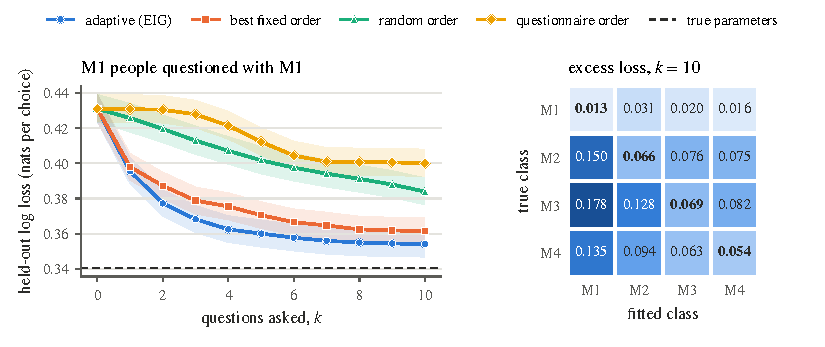
\includegraphics{fig_simulation.pdf}
  \caption{Simulated people. Left: held-out log loss when people simulated from a fitted M1 are questioned with M1, under each selection rule (bands: 95\% intervals; dashed: loss with the true parameters). Right: excess held-out loss over the true parameters after ten adaptive questions, for people simulated from each class (rows) and questioned with each class (columns); the lowest entry in each row is in bold.}
  \label{fig:sim}
\end{figure}

\begin{figure}[t]
  \centering
  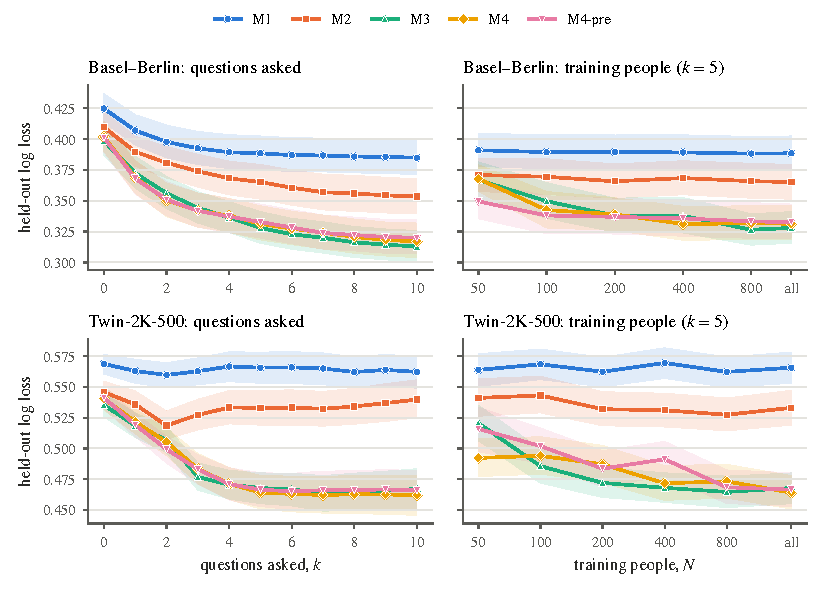
\includegraphics{fig_curves.pdf}
  \caption{Held-out log loss (nats per choice) under adaptive selection on Basel--Berlin (top, prior with the self-rating) and Twin-2K-500 (bottom, no rating). Left: against questions asked, with all training people. Right: after five questions, against the number of training people. Bands are 95\% bootstrap intervals over test people. Every class is scored on the same test people, so the bands have similar widths; differences between classes are tested on paired intervals (Table~\ref{tab:hyp}). Each training size uses one random draw of training people, so the right-hand bands understate the uncertainty at small $N$; Appendix~\ref{app:checks} repeats $N \le 200$ with four more draws.}
  \label{fig:curves}
\end{figure}

\begin{table}[t]
  \caption{The four hypotheses. Loss differences in nats per held-out choice (negative favors the first-named option), AUC differences for H4; 95\% paired bootstrap intervals; the class used is in parentheses.}
  \label{tab:hyp}
  \centering\small
  \begin{tabularx}{\linewidth}{@{}Xll@{}}
    \toprule
    Comparison & Basel--Berlin (exploratory) & Twin-2K-500 (confirmatory) \\
    \midrule
    \tablebody{../code/tables/tab_hypotheses.tex}
    \bottomrule
  \end{tabularx}
\end{table}

\paragraph{Sanity check on simulated people.} When people are simulated from a fitted M1 and M1 is used to question them, adaptive selection does what it should (Figure~\ref{fig:sim}, left): it beats the best fixed order by 0.011 nats per choice at $k = 5$ (95\% interval $[0.008, 0.013]$), its curve comes within 0.014 of the loss with the true parameters after ten questions, and it recovers each person's risk aversion with correlation 0.93 after five questions. On a $4 \times 4$ grid of true by fitted class (Figure~\ref{fig:sim}, right), the true class has the lowest loss after ten questions in every row. Fitting the wrong class costs most when the truth is flexible and the fitted class is not: on people simulated from M2, M3 or M4, M1 is 0.08 to 0.11 nats per choice worse than the true class. M3 and M4 lose little on M1 people (0.007 and 0.003). So the code and the adaptive rule work when the model is right, and a flexible class is the safer guess when the truth is unknown.

\paragraph{H1: flexible models win at every training size.} Figure~\ref{fig:curves} and Table~\ref{tab:hyp} show the opposite of H1. On Basel--Berlin the better simple class is always M2, and M3 and M4 already tie it with 50 training people; from 100 people on they are ahead by 0.02--0.04. Pretraining helps only where data are scarce: M4-pre is the best class at $N \le 200$ (0.349 against 0.371 for M2 at $N = 50$). On Twin-2K-500 every flexible class beats M2 at every $N$, by 0.065--0.069 at full size. A low-rank factor model with two or three dimensions per person, learned from a few hundred people, describes how people answer gamble questions better than either textbook theory. Scaling every list by one constant per dataset instead, so that risk aversion applies to money in the same units throughout, makes M1 and M2 worse, not better (Appendix~\ref{app:checks}). This agrees with \citet{peterson2021} on large data but extends it down to very small samples, possibly because each price list is a narrow family of gambles that a few learned dimensions can cover.

\begin{figure}[t]
  \centering
  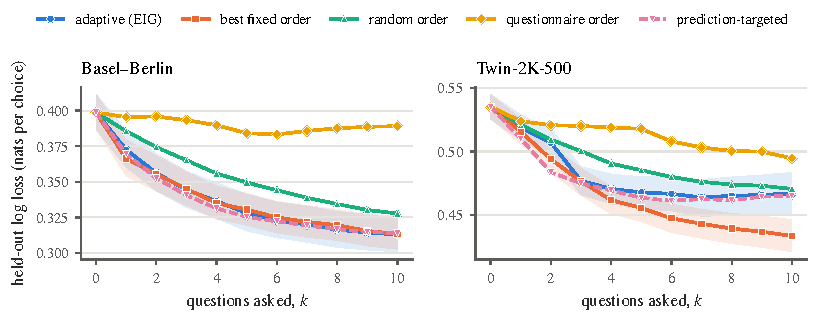
\includegraphics{fig_rules.pdf}
  \caption{Held-out log loss against questions asked under each selection rule, factor model M3 with all training people (Basel--Berlin with the self-rating in the prior, Twin-2K-500 without). Bands: 95\% intervals for the adaptive rule and the best fixed order.}
  \label{fig:rules}
\end{figure}

\paragraph{H2: adaptive questions do not pay off on real people.} Under the class best at full $N$, adaptive selection ties the best fixed order on both datasets (Table~\ref{tab:hyp}, Figure~\ref{fig:rules}). Under the other classes it ties on Basel--Berlin, except M2, where it is worse by 0.014 $[0.007, 0.020]$. On Twin-2K-500 it is worse for M1, M2 and M3 (M3: 0.012 $[0.006, 0.019]$ at $k = 5$, 0.034 $[0.025, 0.042]$ at $k = 10$), and after ten questions it is no better than a random order. The adaptive curve flattens after about four questions while the fixed order keeps improving, and its calibration error grows with $k$ (M3 on Twin-2K-500: 0.011 at $k = 0$, 0.035 at $k = 10$, against 0.012 for the fixed order). Since the same rule works on simulated people, a likely explanation is model error: adaptive questions are chosen where the model expects to learn most, and when the model is wrong the answers there may mislead it, so the posterior becomes confident about the wrong thing. The simulated grid supports this (Table~\ref{tab:grid}): at $k = 10$ adaptive selection beats the best fixed order in all eleven cells where the fitted class is the true one or more flexible (counting M3 and M4 as alike), and in none of the five where it is simpler, where it ties or loses (M2 on M3 people loses by 0.013 $[0.007, 0.019]$ at $k = 5$, about M3's loss on Twin-2K-500). So a wrong model alone can turn the adaptive advantage into a loss. Twin-2K-500 answers are also noisier: its lists are worded as hypothetical (``Suppose you are given the option\ldots'') with no payment, unlike the incentivized Basel--Berlin choices, and M1's fitted lapse rate there is 0.19--0.21 against 0.08--0.09. M3's fitted lapse rate is near zero on both, likely because its per-question offsets absorb inconsistent answers, so a new person's posterior treats every answer as fully informative; forcing $\varepsilon = 0.15$ shrinks the Twin-2K-500 gap (see Robustness). One simpler explanation does not hold: adaptive questions on Twin-2K-500 are not stuck in one list, covering 3.1 distinct price lists in the first five questions on average against 2.0 on Basel--Berlin, where adaptive selection does no harm. Targeting predictions instead of parameters does not fix this: the exploratory prediction-targeted rule ties the parameter-targeted one for every class on both datasets, except M4-pre on Twin-2K-500 at $k = 5$ ($-0.007$ $[-0.014, -0.000]$).

\paragraph{H3: the general self-rating adds little.} On Basel--Berlin, adding the general rating to M3's prior lowers the loss before any question by only 0.0015 nats per choice, already below the 0.01 bar, so by the plan's rule the rating stops helping at $k = 0$. The same holds for every class, and with the financial rating in the prior instead (Appendix~\ref{app:checks}).

\paragraph{H4: lottery answers versus real decisions.} Lottery answers say little about the self-ratings: predicted from the M3 posterior after ten questions, the general rating has an out-of-fold correlation of 0.09 $[0.04, 0.14]$ with its prediction and the financial rating 0.08 $[0.03, 0.14]$ (0.05 to 0.13 across classes). This is not because the gamble answers are unreliable: the shares of risky choices on odd- and even-numbered lists correlate 0.80 (split-half reliability 0.89), and correcting for attenuation (Lecture 14) with that value and the 0.68 mean retest correlation of self-reports in \citet{frey2017} raises 0.09 only to 0.12. The two kinds of measure largely capture different things, so we test each against real decisions. The posterior after ten questions predicts stock investment about as well as the general self-rating (AUC 0.58 against 0.59 for M3; difference $-0.01$ $[-0.14, 0.12]$, a wide interval with 43 investors), so H4 holds on the point estimate. For the equity fund choice it is clearly worse ($-0.10$ $[-0.15, -0.05]$), and adding the posterior to the rating barely helps either outcome. The financial self-rating, a direct question about money, predicts stock investment with AUC 0.88 $[0.83, 0.93]$, far above anything built from gambles. The comparison favors the rating: it and the outcome are self-reports from one session, and recent stock buying may itself raise the rating. This agrees with \citet{frey2017}, who found on the same sample that self-reports relate more strongly than lottery tasks to risk taking outside the laboratory. In the SCF, the rating raises the cross-fitted AUC of a stock-ownership model from 0.752 to 0.774 (difference 0.022 $[0.012, 0.032]$) beyond age, income, wealth and education, with an odds ratio of 1.22 $[1.17, 1.27]$ per point.

\paragraph{Robustness.} Table~\ref{tab:rob} repeats the adaptive--fixed comparison while changing one modeling choice at a time. On Basel--Berlin the adaptive rule stays within 0.011 nats of the best fixed order under every change but one: with the lapse rate set to zero, M1 becomes much worse (0.078 $[0.053, 0.107]$ at $k = 10$), since one stray answer then pushes the posterior to an extreme. On Twin-2K-500, where these runs are exploratory, no change makes adaptive selection beat the fixed order at $k = 10$. The gap shrinks when M3 is allowed more random answers ($\varepsilon = 0.15$: 0.008 $[0.003, 0.012]$) or more dimensions ($K = 5$: 0.008 $[0.003, 0.014]$, with calibration error falling from 0.035 to 0.014), and grows when M1 is given less lapse than it fitted. A weaker or stronger prior changes little. A model that allows for more ways to be wrong is hurt less, as model error predicts, but no change closes the gap.

\begin{table}[t]
  \caption{Robustness of adaptive selection: adaptive minus best fixed order (nats per choice) at $k = 5$ and 10 (with 95\% interval), and the adaptive rule's expected calibration error (ECE) at $k = 10$. The lapse rate and prior scale are changed after fitting (fitted $\varepsilon$: M1 0.08--0.09 on Basel--Berlin, 0.19--0.21 on Twin-2K-500; M3 below 0.001, so it has no $\varepsilon = 0$ row); the rank is fixed before fitting.}
  \label{tab:rob}
  \centering\scriptsize
  \setlength{\tabcolsep}{3pt}
  \begin{tabular}{@{}llllllll@{}}
    \toprule
    & & \multicolumn{3}{c}{Basel--Berlin} & \multicolumn{3}{c}{Twin-2K-500} \\
    \cmidrule(lr){3-5}\cmidrule(l){6-8}
    Class & Check & $k = 5$ & $k = 10$ & ECE & $k = 5$ & $k = 10$ & ECE \\
    \midrule
    \tablebody{../code/tables/tab_robustness.tex}
    \bottomrule
  \end{tabular}
\end{table}

\paragraph{What worked, what did not, and what we learned.} Three things worked: the adaptive rule on simulated people with the right model, flexible models even with little data, and the financial self-rating as a predictor of investment. Adaptive selection on real people did not, and neither the prediction-targeted rule nor any robustness change rescued it. The main lesson for us is that an elicitation rule that succeeds on people simulated from its own model can fail on real people, so it has to be tested on real answers against a strong fixed design, and the model class has to be chosen before the question rule.

\paragraph{What this means for an adviser.} Most of the gain comes from the model of how people answer, learned once from a few hundred people, not from choosing questions for each client. A fixed list chosen on past clients is as good as adaptive questions when the model fits and better when it does not, and it is easier to audit, since every client sees the same questions; adaptive selection is attractive only when the model is trusted. And for the decision an adviser cares about, investing in stocks, a direct question about financial risk did far better than ten gamble answers.

\paragraph{Limitations.} Lottery answers are a proxy for investment decisions, and our samples are Swiss, German and US adults. Candidate questions are limited to those each person answered, so adaptive selection cannot pick a gamble outside the original lists, and M3, which has parameters for each question, could not score a new gamble at all. Held-out lists are whole lists, which makes prediction harder than predicting rows of a list already started, and favors models that share structure across lists. The stock outcome has only 43 positive cases, so the H4 intervals are wide. Our explanation for the failure of adaptive selection, model error, is tested only on simulated people, whose model error is of a known kind. Finally, Basel--Berlin shaped our design choices, and every analysis on Twin-2K-500 other than the single confirmatory run, including the robustness checks, is exploratory.

\section{Conclusion and future work}

The model class mattered more than the selection rule: a factor or neural model learned from as few as 50 to 100 people predicted a new person's choices better than expected utility or prospect theory, while adaptive questions gave no gain over a good fixed list and, on the confirmatory dataset, made predictions worse and overconfident. The general self-rating added little to predicting gambles, but the financial self-rating predicted real investment far better than gambles did. For preference elicitation more broadly, gains from adaptive design on simulated respondents should not be assumed for real ones, and a well-chosen fixed design is the baseline to beat. Future work should try selection rules that account for model error, for example by tempering the posterior, mixing over model classes or planning several questions ahead; and ask whether gamble answers add anything to the financial self-rating for real portfolio decisions.

\bibliographystyle{plainnat}
\bibliography{../refs}

\appendix
\section{Model and fitting details}\label{app:models}
All classes share $P(y_{iq} = 1) = \varepsilon/2 + (1 - \varepsilon)\,\sigma(s_{iq})$ with one lapse rate $\varepsilon$ for the dataset, and outcomes scaled to $[-1, 1]$ within each price list. The rating $z_i$ is centered; without it, the prior mean does not depend on $z_i$.

\paragraph{M1.} $s_{iq} = [\mathrm{EU}(\text{risky}; r_i) - \mathrm{EU}(\text{safe}; r_i)]/\tau$, with $u(x) = (1 - e^{-r x})/r$ ($u(x) = x$ at $r = 0$) and one temperature $\tau$ for all lists. The person parameter $r_i$ lives on 161 equally spaced points in $[-6, 10]$, with prior weights from $\mathcal{N}(\mu_0 + \mu_1 z_i, \sigma^2)$. The five parameters $(\tau, \varepsilon, \mu_0, \mu_1, \sigma)$ maximize the marginal likelihood of the training answers, with $r_i$ summed out on the grid, by L-BFGS-B from the best of 24 starting points.

\paragraph{M2.} Value $v(x) = x^{\alpha}$ for gains and $-\lambda(-x)^{\alpha}$ for losses; weighting $w(p) = p^{\gamma}/(p^{\gamma} + (1-p)^{\gamma})^{1/\gamma}$, one $\gamma$ for gains and losses~\citep{tversky1992}. A two-outcome gamble with outcomes $x_{\mathrm{hi}} > x_{\mathrm{lo}}$ is worth $w(p_{\mathrm{hi}})v(x_{\mathrm{hi}}) + (1 - w(p_{\mathrm{hi}}))v(x_{\mathrm{lo}})$ over gains, $w(p_{\mathrm{lo}})v(x_{\mathrm{lo}}) + (1 - w(p_{\mathrm{lo}}))v(x_{\mathrm{hi}})$ over losses, and $w(p_{\mathrm{hi}})v(x_{\mathrm{hi}}) + w(p_{\mathrm{lo}})v(x_{\mathrm{lo}})$ when mixed; $s_{iq}$ is the difference in value divided by $\tau$. The person parameters $\theta_i = (\log\alpha_i, \log\lambda_i, \log\gamma_i)$ have prior $\mathcal{N}(\mu_0 + \mu_1 z_i, \mathrm{diag}(\sigma^2))$, and $\alpha$, $\lambda$, $\gamma$ are clipped to $[0.05, 3]$, $[0.1, 10]$ and $[0.28, 2.5]$ (the last keeps $w$ increasing). The eleven population parameters are $\tau$, $\varepsilon$ and three each of $\mu_0$, $\mu_1$, $\sigma$. Each of five Monte Carlo EM rounds draws 3,000 points from a normal proposal centered on the current prior (1.5 times its spread, at least 0.15), fits $\tau$ and $\varepsilon$ by L-BFGS-B, and updates the prior in closed form from the people's posterior means and variances. The last round's points carry every posterior as importance weights.

\paragraph{M3.} $s_{iq} = u_i^\top v_q + b_q$, with one vector $v_q \in \mathbb{R}^K$ and offset $b_q$ per question. The scores exist only for questions in the training data, so unlike M1, M2 and M4, M3 cannot score a new gamble. The prior is $\mathcal{N}(c + B z_i, \Sigma)$. Each of four EM rounds maximizes the joint penalized likelihood of $(v, b, u_1, \dots, u_n, \varepsilon)$ by L-BFGS with analytic gradients (penalty $\lambda\lVert v\rVert^2$, offsets unpenalized), then updates $(c, B)$ by least squares of the modes on $[1, z_i]$ and $\Sigma$ from the Laplace covariances and residuals, and finally rewrites the model so that the prior is $\mathcal{N}(B z_i, I)$, which keeps the penalty from being evaded by shrinking $v$. A new person's posterior is a Laplace approximation found by Gauss--Newton steps; predictions and EIG use the linearized score and 20-point Gauss--Hermite quadrature.

\paragraph{M4.} $s_{iq} = w_2^\top \tanh(W_1^{\phi}\phi_q + W_1^{u}u_i + b_1) + b_2$, where $\phi_q$ holds the four payoffs and four probabilities of the two options and $u_i \in \mathbb{R}^2$; 16 hidden units; penalty $\lambda$ on $W_1^{\phi}$, $W_1^{u}$ and $w_2$. During fitting each training person has a Gaussian variational posterior with diagonal covariance, its expectation taken over four fixed antithetic draws, and the same three-round EM as M3 (L-BFGS, at most 300 iterations per round). A new person's posterior is held as importance weights on 4,000 shared draws from a normal proposal 1.5 times as wide as the prior. M4-pre first fits M2 to the same training people, simulates 2,000 people from it who answer every question, fits the network to them ($\lambda = 0.1$), and then fits the real people with the penalty $\lambda\lVert w - w_{\mathrm{pre}}\rVert^2$.

\paragraph{Hyperparameters.} The rank and penalties are chosen on a validation fifth of the training people, each with two held-out lists, by the mean held-out loss over $k = 0, \dots, 10$ random questions.

\section{Further checks}\label{app:checks}
These checks were not in the plan and are exploratory.

\paragraph{Accuracy.} Table~\ref{tab:acc} gives the share of held-out choices predicted correctly. It ranks the classes as log loss does, and adaptive and fixed orders differ by less than one percentage point except on Twin-2K-500 at $k = 10$, where the fixed order is ahead for M1 (by 1.6 points) and M3 (0.9).

\begin{table}[h]
  \caption{Held-out accuracy after $k$ questions, adaptive (A) and best fixed order (F), prior as in deployment.}
  \label{tab:acc}
  \centering\small
  \begin{tabular}{@{}lllllllll@{}}
    \toprule
    & \multicolumn{4}{c}{Basel--Berlin} & \multicolumn{4}{c}{Twin-2K-500} \\
    \cmidrule(lr){2-5}\cmidrule(l){6-9}
    & A, $k = 5$ & F, $k = 5$ & A, $k = 10$ & F, $k = 10$ & A, $k = 5$ & F, $k = 5$ & A, $k = 10$ & F, $k = 10$ \\
    \midrule
    \tablebody{../code/tables/tab_accuracy.tex}
    \bottomrule
  \end{tabular}
\end{table}

\paragraph{Fixed order on simulated people.} Table~\ref{tab:grid} adds the best fixed order to the $4 \times 4$ grid of Figure~\ref{fig:sim} and gives adaptive minus fixed under each pair of true and fitted class.

\begin{table}[h]
  \caption{Simulated people: adaptive minus best fixed order (nats per choice, 95\% interval) by true class (rows) and fitted class (columns). Negative values favor adaptive selection.}
  \label{tab:grid}
  \centering\scriptsize
  \setlength{\tabcolsep}{3pt}
  \begin{tabular}{@{}llllll@{}}
    \toprule
    & True & Fitted M1 & Fitted M2 & Fitted M3 & Fitted M4 \\
    \midrule
    \tablebody{../code/tables/tab_grid_rules.tex}
    \bottomrule
  \end{tabular}
\end{table}

\paragraph{Payoff scale.} The main analysis scales each price list to $[-1, 1]$ by its own largest stake, although Basel--Berlin stakes range from 3.85 to 200 in the study's currency. Dividing all outcomes by one constant per dataset, its largest stake, makes M1 worse on Basel--Berlin by 0.044 $[0.037, 0.052]$ nats per choice before any question and by 0.117 $[0.102, 0.132]$ after five adaptive questions, and M2 worse by 0.018 $[0.015, 0.021]$ and 0.006 $[-0.002, 0.014]$. On Twin-2K-500, whose stakes vary less (6 to 20 dollars), the change is small: before any question M1 improves by 0.004 $[0.002, 0.005]$ and M2 worsens by 0.001, under the best fixed order both stay within 0.01 of the main run, and under adaptive selection both get worse (by 0.034 and 0.028 at $k = 5$). None of this approaches the 0.065 gap to the flexible classes, so per-list scaling does not handicap the simple classes in H1.

\paragraph{More draws of training people.} Repeating $N = 50$, 100 and 200 with four more random draws of training people (adaptive selection, $k = 5$) leaves H1 unchanged. On Twin-2K-500, and from $N = 100$ on Basel--Berlin, every flexible class beats the better simple class (M2) in all five draws. At $N = 50$ on Basel--Berlin, M4-pre is ahead in every draw, but M3 is behind M2 in three draws (by up to 0.027) and M4 in one, so their tie with M2 at $N = 50$ holds only on average (mean over draws: M3 $+0.004$ $[-0.004, 0.013]$, M4 $-0.009$ $[-0.015, -0.002]$).

\paragraph{Financial rating in the prior.} Replacing the general rating with the financial one in the Basel--Berlin prior changes the adaptive loss of M1, M2 and M3 by at most 0.003 at $k = 0$, 5 and 10, and it never beats the prior without any rating by more than 0.001.

\newpage
\newcommand{\finalonly}[1]{#1}
% The three required disclosures (about 150 words each), shared by the pre-analysis plan and the final manuscript.
% \finalonly{...} text appears only in the final manuscript, which defines it before this file.
\providecommand{\finalonly}[1]{}
\section*{Required statements}

\subsection*{Integrity statement}
Plagiarism of text: every source we draw on is cited, nothing is copied without quotation marks, and references were checked against OpenAlex. Plagiarism of ideas: borrowed methods are credited where they appear (BALD, DOSE, cognitive-model pretraining), and all code is our own. Bias: we fixed hypotheses and decision rules before running experiments, list every deviation, and report each dataset separately because the samples are Swiss, German and US adults. Inaccuracies: the public Basel--Berlin file codes 0--10 ratings as 1--11, which we correct; Basel--Berlin informed our design, so its results are exploratory, and Twin-2K-500 was analyzed once, as the confirmatory test.\finalonly{ Selective reporting: results that went against our hypotheses, H1 and H2, are reported as fully as those that supported them, and every number, figure and table in the paper is produced by the submitted code from the public data.}

\subsection*{AI use reflection}
We used Claude Opus 5.5 to search the literature, draft and debug analysis code, and edit our writing. We used it because it made routine work such as data loading and plotting much faster, leaving time to compare four model classes. The research question, model classes, hypotheses and decision rules are ours, and we reviewed all code and text before using it. The tool also made confident errors, so every citation was checked against OpenAlex and every number comes from code we ran. For our learning, checking its output pushed us to work through expected information gain and identification ourselves; the risk is accepting code we do not understand, which we guard against by reading and testing each function. In the future we would ask AI tools to critique a design before we build it, and the course could ask students to submit their AI transcripts with their code.

\subsection*{Impact statement}
Fewer, better-chosen questions could make risk profiling quicker and more accurate, so clients who would skip a long questionnaire still get advice that fits them. The methods could be misused: an adaptive questionnaire could be steered to label clients more risk tolerant than they are, or to profile them for marketing. Mitigations are to publish the question-selection rule and the model, keep the self-rating as a cross-check, and let clients see and correct their profile; our code is submitted for audit. Lottery choices are only a proxy for portfolio decisions, our samples are Swiss, German and American, and adaptive questions made predictions overconfident on one dataset, so the findings are not ready for use with real clients. We collect no new data: all datasets are public and de-identified, used under their licenses and cited, as Stanford's integrity standards require. Everything runs on a laptop, so the environmental cost is negligible.



\end{document}
